\documentclass{article}

\usepackage{ctex}
\usepackage[top=0.7in,bottom=0.7in,left=0.5in,right=0.5in]{geometry}
\usepackage{array}
\usepackage{multirow}
\usepackage{graphicx}
\usepackage{fancyhdr}
\usepackage{lastpage}
\usepackage{extramarks}
\usepackage{amsmath}
\usepackage{listings}
\usepackage{fontspec}
\newfontfamily\consolas{Consolas}
\usepackage{xcolor} % 定制颜色
\definecolor{mygreen}{rgb}{0,0.6,0}
\definecolor{mygray}{rgb}{0.5,0.5,0.5}
\definecolor{mymauve}{rgb}{0.58,0,0.82}
\lstset{ %
backgroundcolor=\color{white},      % choose the background color
basicstyle=\footnotesize\ttfamily,  % size of fonts used for the code
columns=fullflexible,
tabsize=4,
breaklines=true,               % automatic line breaking only at whitespace
captionpos=b,                  % sets the caption-position to bottom
commentstyle=\color{mygreen},  % comment style
escapeinside={\%*}{*)},        % if you want to add LaTeX within your code
keywordstyle=\color{blue},     % keyword style
stringstyle=\color{mymauve}\ttfamily,  % string literal style
frame=single,
rulesepcolor=\color{red!20!green!20!blue!20},
% identifierstyle=\color{red},
language=c++,
}

\newcommand{\hmwkTitle}{2/8进制转换器\ 实验报告}
\newcommand{\hmwkClass}{数据结构}
\newcommand{\hmwkClassInstructor}{}
\newcommand{\hmwkAuthorName}{毛子恒\ 李臻\ 张梓靖}

\pagestyle{fancy}
\lhead{\hmwkAuthorName}
\chead{\hmwkClass\ : \hmwkTitle}
\rhead{\firstxmark}
\lfoot{\lastxmark}
\cfoot{\thepage}
\renewcommand\headrulewidth{0.4pt}
\renewcommand\footrulewidth{0.4pt}

\title{\hmwkClass\ :\hmwkTitle}
\author{\hmwkAuthorName}

\setcounter{tocdepth}{1}

\begin{document}

\maketitle  

\section*{小组成员}

\setlength{\tabcolsep}{9mm}
{
    \begin{table}[htbp]
        \centering
        \begin{tabular}{llll}
            班级:2019211309 & 姓名:毛子恒 & 学号:2019211397 & 分工:代码\ 文档 \\
            
            班级:2019211310 & 姓名:李臻   & 学号:2019211458 & 分工:测试\ 文档 \\
            
            班级:2019211308 & 姓名:张梓靖 & 学号:2019211379 & 分工:文档       \\
        \end{tabular}
    \end{table}
}

\tableofcontents
\newpage

\section{需求分析}

\subsection{题目描述}

输入一串二进制数,输出其八进制表示。

\subsection{输入描述}

程序从标准输入中读入数据。输入一个0/1串表示二进制数,以“\#”表示输入结束。

输入满足二进制串的长度$LEN\leq 10^6$

\subsection{输出描述}

程序向标准输出中输出结果。

输出分为三种情况:

\begin{enumerate}
    \item 输入合法,程序正常运行结束。此时输出一行一个八进制数。
    \item 输入不合法,即输入中包含除了0/1、空白字符、\#以外的其他字符,此时输出一行一个字符串"Please check your input."(不带引号)。
    \item 程序发生运行时错误,比如内存分配失败。此时程序没有输出。
\end{enumerate}

\subsection{样例输入输出}

\subsubsection{样例输入输出1}

【输入】

\begin{lstlisting}[
    basicstyle=\small\consolas]
110#
\end{lstlisting}

【输出】

\begin{lstlisting}[
    basicstyle=\small\consolas]
6
\end{lstlisting}

\subsubsection{样例输入输出2}

【输入】

\begin{lstlisting}[
    basicstyle=\small\consolas]
010111111#
\end{lstlisting}

【输出】

\begin{lstlisting}[
    basicstyle=\small\consolas]
277
\end{lstlisting}

\subsubsection{样例输入输出3}

【输入】

\begin{lstlisting}[
    basicstyle=\small\consolas]
0110001010#
\end{lstlisting}

【输出】

\begin{lstlisting}[
    basicstyle=\small\consolas]
612
\end{lstlisting}

\subsubsection{样例输入输出4}

【输入】

\begin{lstlisting}[
    basicstyle=\small\consolas]
1101000110010000000101000101100100100001011100110111111111010000001011000101111100010100011100#
\end{lstlisting}

【输出】

\begin{lstlisting}[
    basicstyle=\small\consolas]
15062005054441346777201305742434
\end{lstlisting}

\subsubsection{样例输入输出5}

【输入】

\begin{lstlisting}[
    basicstyle=\small\consolas]
112000#
\end{lstlisting}

【输出】

\begin{lstlisting}[
    basicstyle=\small\consolas]
Please check your input.
\end{lstlisting}

\subsection{程序功能}

程序将输入的二进制串转化为八进制并且输出。

\section{概要设计}

\subsection{问题解决的思路}

使用栈模拟操作过程。首先将所有二进制位依次入栈$s1$。之后每次从$s1$栈顶取出三个二进制位,将其转化为一个八进制位后入栈$s2$,最后把$s2$中元素依次出栈并输出。

此题中栈实现了初始化、判空、入栈、出栈、获取栈顶元素、释放空间这六种操作。

\subsection{栈的定义}

\begin{lstlisting}[language={C},
    numbers=left,
    numberstyle=\tiny\consolas,
    basicstyle=\small\consolas]
//数据对象
typedef struct stack
{
    ElemType * top;
    ElemType * base;
    int stacksize;
} Stack;

/*
 * 操作:初始化栈,分配空间
 * 后件:s指向一个空栈
 */
void initStack(Stack * s);

/*
 * 操作:判断栈是否为空
 * 前件:s是一个栈
 * 后件:如果该栈为空,返回true;否则返回false
 */
bool isStackEmpty(Stack s);

/*
 * 操作:将数据元素入栈
 * 前件:s指向一个栈
 * 后件:如果入栈成功,item成为栈顶元素;如果入栈之前该栈已满,则重新分配空间
 */
void pushStack(Stack * s, ElemType item);

/*
 * 操作:获取栈顶元素
 * 前件:s是一个栈
 * 后件:如果该栈不为空,返回栈顶元素
 */
ElemType getStackTop(Stack s);

/*
 * 操作:栈顶元素出栈
 * 前件:s指向一个栈
 * 后件:如果该栈不为空,栈顶元素出栈,返回这个出栈的元素
 */
ElemType popStack(Stack * s);

/*
 * 操作:释放栈空间
 * 前件:s指向一个栈
 * 后件:释放该栈的空间
 */
void destroyStack(Stack * s);
\end{lstlisting}

\subsection{主程序的流程}

\begin{enumerate}
    \item 初始化栈
    \item 输入,元素入$s1$栈
    \item 每次从$s1$中出栈三个元素,计算对应的八进制位并入$s2$栈,重复执行直到$s1$为空
    \item 元素出$s2$栈并输出
    \item 释放空间
\end{enumerate}

\subsection{各程序模块之间的层次关系}

函数调用关系图如图1。

\begin{figure}[htbp]
    
    \centering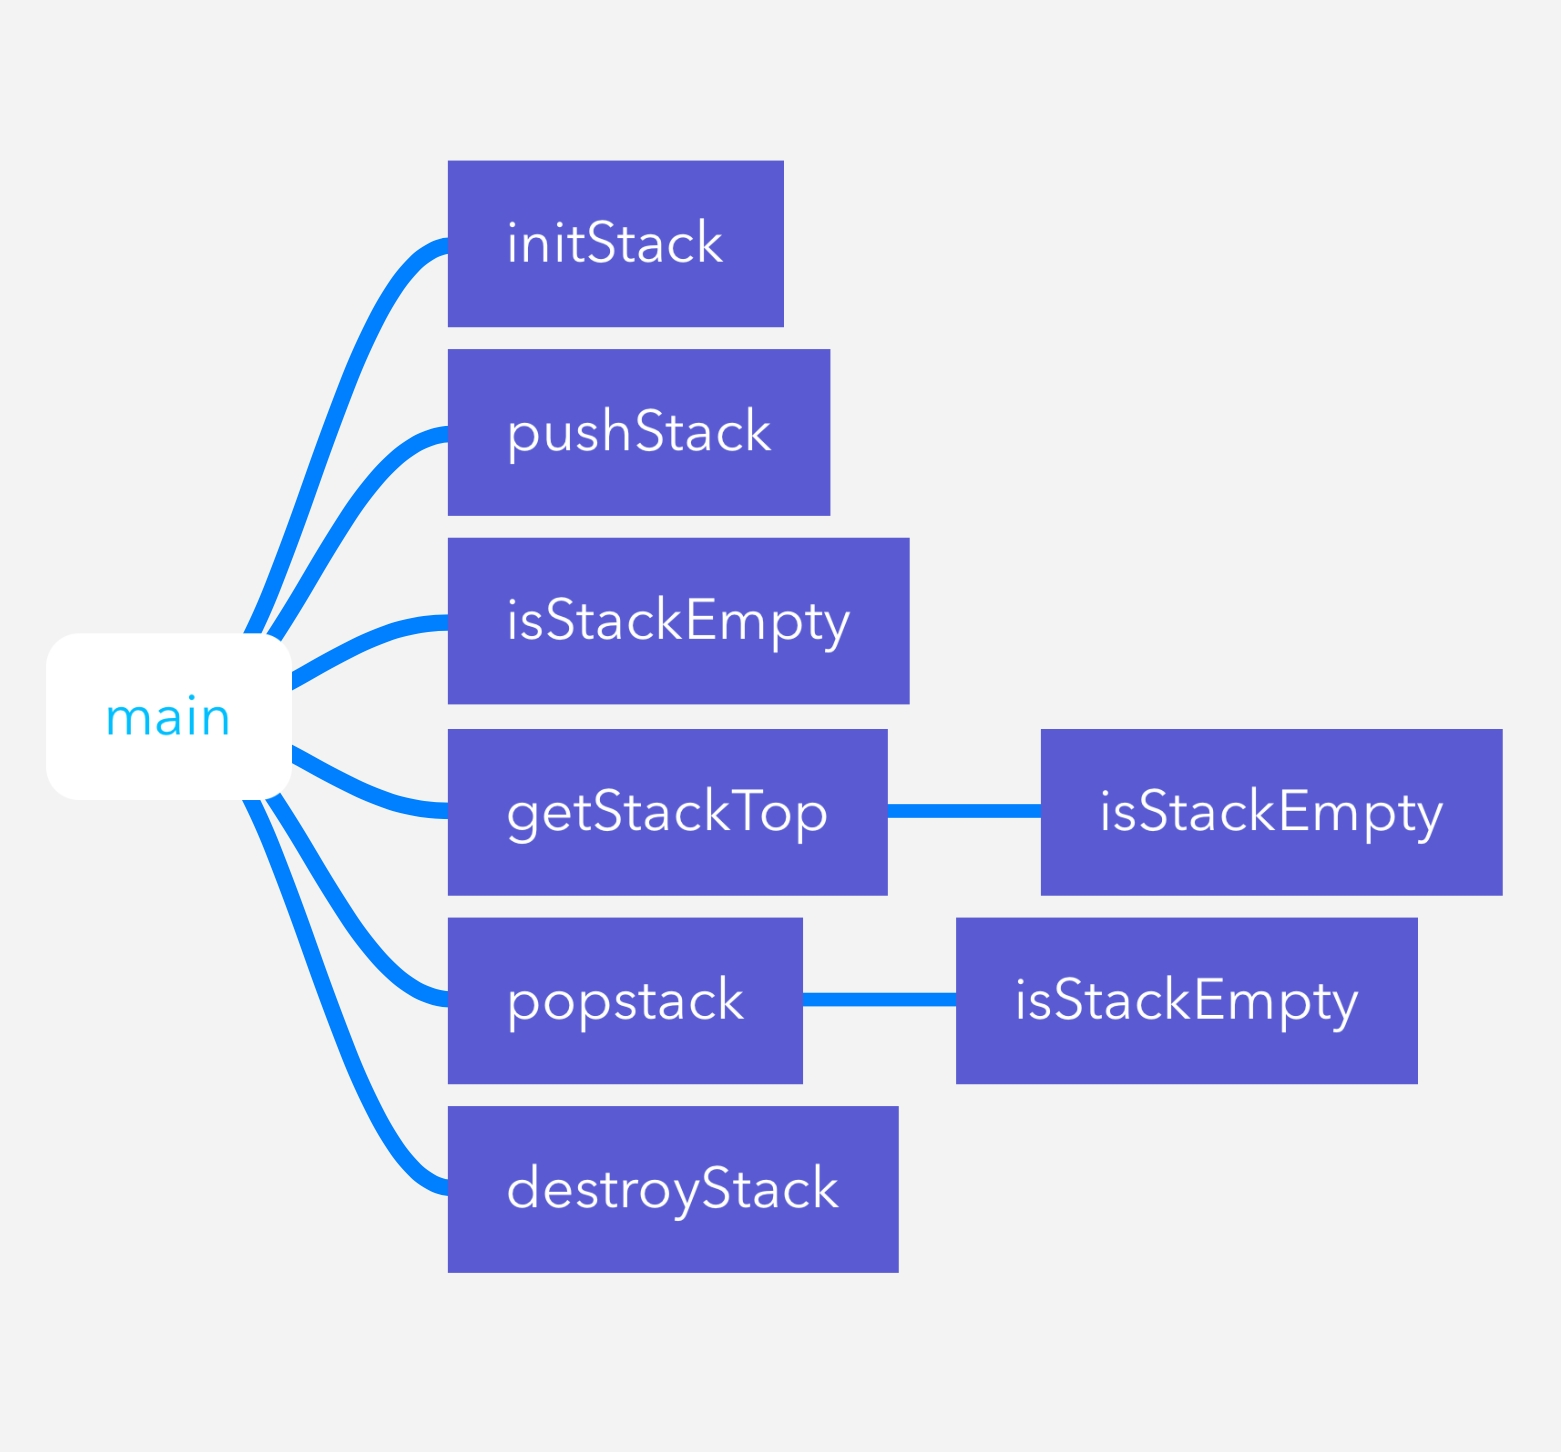
\includegraphics[width=0.4\textwidth]{./Images/pic2_1.png}
    
    \caption{函数的调用关系}
    
\end{figure}

\section{详细设计}

\subsection{栈的实现}

链表设计中基本操作的伪代码算法如下:
\begin{lstlisting}[language={C},
    numbers=left,
    numberstyle=\tiny\consolas,
    basicstyle=\small\consolas]
void Stack(Stack * s) // 初始化链表
{    
    给*s分配内存
    if (*s内存分配失败)// 空间分配失败
        异常退出
    s->top <- s->base
    s->stacksize <- STACKINCREASESIZE
}

bool isStackEmpty(Stack s)// 判断栈是否为空
{
    if (s栈为空) 返回1
    else 返回0
}

void pushStack(Stack * s, ElemType item)// 将数据元素入栈
{
    if (s栈满) 
    {
        分配给s更多的空间
        if (s空间分配失败)
            异常退出
        s->top <- s->base + s->stacksize
        s->stacksize 增加 STACKINCREASESIZE 的空间
    }
    item入栈
}

ElemType getStackTop(Stack s)// 获取栈顶元素
{
    if (栈为空)
        返回异常
    返回 *(s.top - 1)
}

ElemType popStack(Stack * s)// 栈顶元素出栈
{
    if (栈为空)
        返回异常 
    返回 *(--s->top)
}

void destroyStack(Stack * s)// 释放栈空间
{
    释放s->base
    s->base <- NULL
    s->top <- NULL
    s->stacksize <- 0
}
\end{lstlisting}

\subsection{函数的调用关系图}

如2.4所示。

\section{调试分析报告}

\subsection{调试过程中遇到的问题和思考}

初步实现后,测试样例时发现对于前导零的情况没有处理,遂增加查询栈顶操作,并且在主程序中增加弹出栈顶0元素的循环。

之后对串全为0的情况增加特判。

对于规模较大的数据测试时发现指针会访问到无效位置,发现是realloc操作之后没有更新$top$指针的位置所致。遂增加更新$top$指针的语句。

\subsection{设计实现的回顾讨论}

$Stack$类型的$top$指针指向栈顶元素的下一个位置,实现时有几次没有注意到这个问题而导致错误。

期望输入合法,所以对于更多的不合法输入(比如输入末尾没有\#)没有作处理。

由于不清楚测试用数据的范围大小,$STACKINCREASESIZE$常量的大小取到100,也就是每次增加100个元素的空间。当输入很大时复杂度可能会比较大。

由于主函数对函数的调用足够严密,所以栈 的实现没有考虑不符合前件的情况。

\subsection{算法复杂度分析}

initStack, isStackEmpty, pushStack, getStackTop, popStack, destroyStack函数的时间复杂度均为$O(1)$。

主程序复杂度为$O(n)$,整体时间复杂度为$O(n)$。

\subsection{改进设想的经验和体会}

\subsubsection{改进1}

程序中的各个栈操作都可以直接改成一个数组的正序/逆序的访问。但是空间浪费很严重。并且不符合题目要求。

\section{用户使用说明}

使用gcc编译生成可执行文件。

\begin{lstlisting}[language={bash},
    basicstyle=\small\consolas]
gcc -o main -std=c11 main.c stack.c
\end{lstlisting}

执行可执行文件:

\begin{lstlisting}[language={bash},
    basicstyle=\small\consolas]
./main
\end{lstlisting}

在Windows cmd下:

\begin{lstlisting}[language={bash},
    basicstyle=\small\consolas]
main
\end{lstlisting}

之后通过标准输入输入数据,输入格式参考1.2节的输入描述,结果通过标准输出返回。如果输入合法并且程序正常运行结束,主函数返回值为0。

\section{测试结果}

测试环节分为三个步骤。

\subsection{测试第一部分}

对1.4节给出的样例进行测试。

\subsection{测试第二部分}

测试非法输入和边界条件。

【输入】

\begin{lstlisting}[language={bash},
    basicstyle=\small\consolas]
5 -1 2
\end{lstlisting}

【输出】

\begin{lstlisting}[language={bash},
    basicstyle=\small\consolas]
Please check your input.
\end{lstlisting}

\subsection{测试第三部分}

使用Python实现2/8进制转换器(test.py)如下:

\begin{lstlisting}[language={Python},
    numbers=left,
    numberstyle=\tiny\consolas,
    basicstyle=\small\consolas]
a = int(input()[:-1], 2)
print(oct(a)[2:])
\end{lstlisting}

将原解法与此解法比对。

测试在macOS\ Catalina\ 10.15.6下进行。

在$LEN<=10$,$LEN<=1000$,$LEN<=1000000$的范围下分别随机生成1000组测试数据,分别传入main和test.py,并且比对两程序的输出。

3000组数据中两程序的输出均相同。

数据生成程序(data.cpp)如下:

\begin{lstlisting}[language={C++},
    numbers=left,
    numberstyle=\tiny\consolas,
    basicstyle=\small\consolas]
#include <bits/stdc++.h>

using namespace std;

const int LEN = 1e4;

int main()
{
    srand(time(0));
    int n = rand() % LEN + 1;
    for (int i = 1; i <= n; ++i)
        printf("%d", rand() % 2);
    puts("#");
    return 0;
}
\end{lstlisting}

比对脚本(chk.sh)如下:

\begin{lstlisting}[language={C++},
    numbers=left,
    numberstyle=\tiny\consolas,
    basicstyle=\small\consolas]
for i in {1..100}
do
    sleep 1
    ./data >in.in
    ./main <in.in >out.out
    python ./test.py <in.in >out1.out
    if ! diff out.out out1.out
    then
        break
    fi
    echo "Correct"
done
\end{lstlisting}

\end{document}
